\chapter{DESARROLLO DEL PROYECTO}
\section{Planificación del proyecto}

El proyecto se desarrolló a lo largo de tres meses, entre junio y agosto de 2026, mediante fases consecutivas e incrementales. El esfuerzo total fue de 330 horas, a un ritmo aproximado de 28 horas semanales (112 horas mensuales). La Tabla~\ref{tab:planificacion} recoge el cronograma con las actividades realizadas y su esfuerzo.

\begin{table}[ht!]
  \centering
  \small
  \begin{tabular}{|p{4.3cm}|p{1.7cm}|c|p{5.8cm}|}
    \hline
    \textbf{Actividad} & \textbf{Periodo} & \textbf{Horas} & \textbf{Entregable} \\ \hline
    Estudio de los antecedentes y estado del arte & Jun. 2026 & 30 & Revisión bibliográfica \\ \hline
    Búsqueda y adaptación de la fuente de datos; establecimiento de objetivos & Jun. 2026 & 5 & \texttt{prepare\_ashrae.py}, objetivos y KPIs \\ \hline
    Selección de herramientas y diseño de la arquitectura & Jun. 2026 & 5 & Documento de diseño \\ \hline
    Desarrollo técnico y pruebas iniciales de la sección de procesamiento & Jun.--Jul. 2026 & 80 & Artefactos en \texttt{bridge/}, \texttt{common/}, \texttt{docker/}, \texttt{schemas/}, \texttt{simulator/} y \texttt{spark/} \\ \hline
    Validación, pruebas y ajustes de la sección de procesamiento & Jul. 2026 & 100 & Informe de resultados: pérdida de mensajes (0,0000\,\%), latencia de ingesta p50/p95 (0,766 / 1,277 s), throughput bajo carga y degradación (652 sensores concurrentes, degradación real 0,6\,\%), tiempo de recuperación ante fallo (4,1 s TimescaleDB / 5,1 s PostgreSQL) \\ \hline
    Creación, pruebas y ajustes de la sección de visualización & Jul.--Ago. 2026 & 30 & Artefactos en \texttt{grafana/} y \texttt{powerbi/} \\ \hline
    Creación y prueba de scripts auxiliares & Ago. 2026 & 5 & Artefactos en \texttt{tools/} y \texttt{setup.sh} \\ \hline
    Redacción de la memoria & Jun.--Ago. 2026 & 75 & Este documento \\ \hline
    \textbf{Total} & & \textbf{330} & \\ \hline
  \end{tabular}
  \caption{Cronograma y esfuerzo de las actividades del proyecto}
  \label{tab:planificacion}
\end{table}

\section{Descripción de la solución, metodologías y herramientas empleadas}

\subsection{Visión general de la arquitectura}

El sistema implementa una arquitectura Kappa de flujo único con una bifurcación final hacia dos consumidores especializados, tal y como muestra la Figura~\ref{fig:arquitectura-tfm}. Cada componente es un servicio independiente, desplegado en su propio contenedor Docker, y la comunicación entre ellos ocurre exclusivamente a través de Kafka como registro reproducible, salvo la gobernanza de esquemas, que se resuelve aparte.

\begin{figure}[ht!]
  \centering
  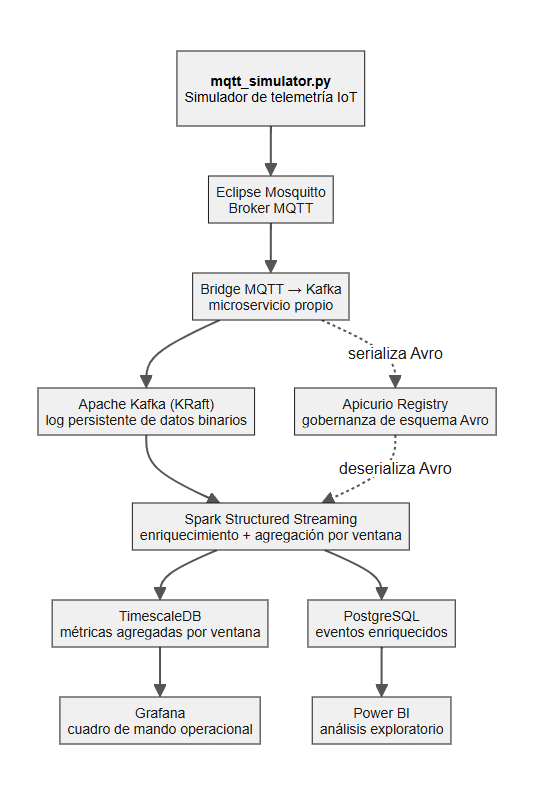
\includegraphics[width=0.85\textwidth]{imagenes/tfm_arquitectura.png}
  \caption[Arquitectura del pipeline IoT]{Arquitectura del sistema: flujo único Kappa (simulador, Mosquitto, bridge, Kafka, Spark) con bifurcación hacia el doble sumidero operacional y analítico. Elaboración propia.}
  \label{fig:arquitectura-tfm}
\end{figure}

El simulador (\texttt{mqtt\_simulator.py}) publica telemetría hacia Eclipse Mosquitto, que actúa únicamente como broker de ingesta MQTT. El bridge, un microservicio propio, suscribe los mensajes, los serializa contra Apicurio Registry conforme al esquema Avro vigente y los publica en Kafka. Es importante notar que Kafka no participa en la gobernanza de esquemas: almacena únicamente un log persistente de bytes opacos, sin conocimiento de su estructura interna; es el bridge, en la escritura, y Spark Structured Streaming, en la lectura, quienes dialogan directamente con Apicurio para serializar y deserializar cada evento respectivamente.

Spark Structured Streaming consume el flujo, enriquece cada evento mediante \textit{join} con las tablas de referencia del edificio y del sensor, y ejecuta dos consultas de streaming independientes sobre el mismo tópico: una agrega métricas por ventana temporal hacia TimescaleDB para su consumo operacional en Grafana, y otra persiste eventos enriquecidos hacia PostgreSQL para su consumo analítico en Power BI. Al tratarse de consultas independientes, cada una mantiene su propio \textit{checkpoint} y su propia tolerancia a fallos, de modo que la caída de un sumidero no interrumpe al otro (sección~\ref{sec:validacion-procesamiento}).
\section{Recursos requeridos}
En este apartado debes enumerar los recursos que has utilizado para la ejecución del proyecto (recursos técnicos, dispositivos, material de laboratorio, asistencia de expertos, etc.). Si bien, en la sección donde se describe Metodología y Herramientas empleadas, se describen en detalle las mismas, en esta sección, únicamente debes enumerarlas.
\section{Presupuesto}
El Presupuesto supone la evaluación económica total del proyecto.
No olvides que tu tiempo también vale dinero, no sólo hay que incluir el coste de los materiales empleados.
A continuación, se muestra un ejemplo de resumen de presupuesto. Puedes añadir entradas a esta tabla si lo necesitas, conforme a la naturaleza de tu trabajo. Todos los recursos requeridos indicados en el apartado anterior deberían estar recogidos en la tabla de costes, aunque hayan tenido coste cero.
\begin{table}[ht!]
  \centering
  \label{tab:costes}
  \begin{tabular}{|l|c|p{6cm}|}
    \hline
    \textbf{Tipo de coste} & \textbf{Valor} & \textbf{Comentarios} \\ \hline
    Horas de trabajo en el proyecto & [Número de horas] & Añade entradas para otras personas que hayan participado en tu proyecto para contabilizar sus horas aproximadas. \\ \hline
    Equipo técnico utilizado & € & Si el equipo no lo has tenido que adquirir, indica su valor aproximado en el mercado si lo tuvieras que adquirir nuevo. Utiliza una entrada en la tabla por cada equipo (desktop, servidor, etc.) \\ \hline
    Software utilizado & € & Si el Software no lo has tenido que adquirir, indica su valor aproximado en el mercado si lo tuvieras que adquirir. Indica coste 0€ si es Software que no requiere pagar precio por licencia. Ejemplos: IDE de desarrollo, herramienta de análisis de datos, programa de diseño gráfico, etc. \\ \hline
    Estudios e informes & € & Si has tenido que adquirir algún informe de consultora o de revista de investigación, indica el coste. \\ \hline
    Materiales empleados & € & P. ej.: material de laboratorio, sensores, etc. \\ \hline
  \end{tabular}
    \caption{Costes del proyecto}
\end{table}

\begin{figure}[ht!]
\centering
\includegraphics[width=0.5\textwidth]{imagenes/logo_ue.png} % Ajusta el nombre y la ruta de tu imagen
\caption{Esta es una imagen de ejemplo.} % Aquí va la leyenda de tu imagen
\label{fig:miImagen} % Etiqueta para referenciar la figura en el texto
\end{figure}

\section{Viabilidad}
Este apartado es opcional, pero es interesante que incluyas un breve análisis de viabilidad económica del proyecto (relación coste / beneficio), y un análisis de sostenibilidad a futuro del resultado de tu proyecto.
\section{Resultados del proyecto}
Conforme a los objetivos específicos, describe los resultados finales obtenidos.
Para proyectos con un enfoque de desarrollo de producto, debes incluir el resultado de tu plan de pruebas.
Puedes añadir una descripción de cambios durante el proyecto respecto a los objetivos iniciales, y comentarios que quieras incluir de cómo has desarrollado las distintas actividades.
